\documentclass{article}
\usepackage{amsmath, amssymb} % Required for math symbols and additional symbols
\usepackage[paper=letterpaper,
           hmargin={1in,1in},
           vmargin={1in,1in},
           ]{geometry}   % Allows you to change the margin sizes
\usepackage{enumitem}  % Required to re-label lists
\usepackage{tikz}      % Required for creating graphics

\title{Prep Work 12}
\author{Xander} 
\date{Mar 26}

\begin{document}

\maketitle
\noindent\textbf{Presentation: } 

I don't really understand these problems. I tried solving them and ended up in a mess of not knowing if im right or not.
I'm going to submit this PW blank and see if I can solve them once I know a bit more.
%%%%%%%%%%%%%%%%% Don't delete anything above this line!

\section*{Exercise 3 4.1}  

Is it possible for two \emph{different} (non-isomorphic) graphs to have the same number of vertices and the same number of edges? What if the degrees of the vertices in the two graphs are the same (so both graphs have vertices with degrees 1, 2, 2, 3, and 4, for example)? Draw two such graphs or explain why not.

\vspace{0.5cm}
\noindent\textbf{Solution Draft:} 
\vspace{0.2cm}



%%%%%%%%%%%%%%%%%%%%%%%%%%%%%%%%%%%%
\section*{Exercise 5 4.1}  

Consider the following two graphs:%
\begin{description}
\item[{\(G_1\)}]\(V_1=\{a,b,c,d,e,f,g\}\)%
\par
\(E_1=\{\{a,b\},\{a,d\},\{b,c\},\{b,d\},\{b,e\},\{b,f\},\{c,g\},\{d,e\}\),%
\par
\(\{e,f\},\{f,g\}\}\).%
\item[{\(G_2\)}]\(V_2=\{v_1,v_2,v_3,v_4,v_5,v_6,v_7\}\),%
\par
\(E_2=\{\{v_1,v_4\},\{v_1,v_5\},\{v_1,v_7\},\{v_2,v_3\},\{v_2,v_6\}\),%
\par
\(\{v_3,v_5\},\{v_3,v_7\},\{v_4,v_5\},\{v_5,v_6\},\{v_5,v_7\}\}\)%
\end{description}
%
\begin{enumerate}[label= (\alph*)]
\item{}Let \(f:G_1 \rightarrow G_2\) be a function that takes the vertices of Graph 1 to vertices of Graph 2. The function is given by the following table:%
\begin{center}
\begin{tabular}{llllllll}
\textbf{x}&\(a\)&\(b\)&\(c\)&\(d\)&\(e\)&\(f\)&\(g\)\\
\hline
\textbf{f (x)}&\(v_4\)&\(v_5\)&\(v_1\)&\(v_6\)&\(v_2\)&\(v_3\)&\(v_7\)
\end{tabular}
\end{center}
%
Does \(f\) define an isomorphism between Graph 1 and Graph 2?%
\item{}Define a new function \(g\) (with \(g \ne f\)) that defines an isomorphism between Graph 1 and Graph 2.%
\item{}Is the graph pictured below isomorphic to Graph 1 and Graph 2? Explain.%
\begin{center}
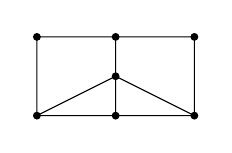
\begin{tikzpicture}
    % Define the vertices as small circles for clarity
    \def\v{circle(0.05) node{}}
	\draw (-1, 0) coordinate (v1) -- (0,0) coordinate (v2) -- (1,0) coordinate (v3) -- (1,1) coordinate (v4) -- (0,1) coordinate (v5) -- (-1,1) coordinate (v6) -- (v1) --(0,.5) coordinate (v7) -- (v2) (v7) -- (v3) (v7) -- (v5);
	\foreach \i in {1,...,7}{
		\fill (v\i) \v;
	}
\end{tikzpicture}
\end{center}
\end{enumerate}

\vspace{0.5cm}
\noindent\textbf{Solution Draft:} 
\vspace{0.2cm}



%%%%%%%%%%%%%%%%%%%%%%%%%%%%%%%%%%%%
\section*{Exercise 7 4.1}  

Which of the graphs below are bipartite? Justify your answers.%
\begin{center}
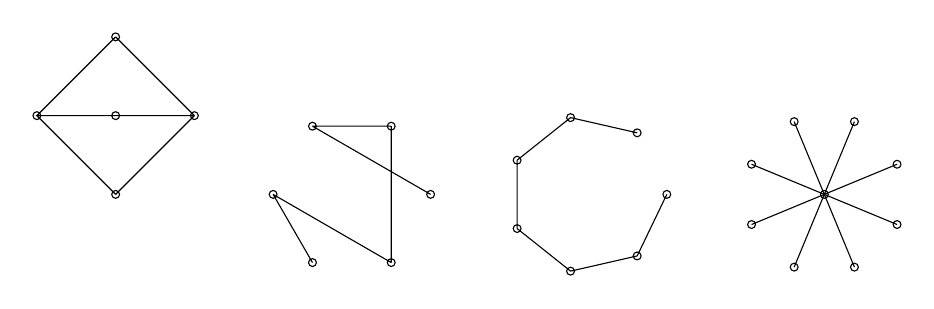
\begin{tikzpicture}
    \def\v{circle(0.05) node{}}
    \begin{scope}[xshift=-3cm]
        \draw (-1,1) \v -- (0,2) \v -- (1,1) \v -- (0,0) \v -- (-1,1) -- (0,1) \v -- (1,1);
    \end{scope}
    \begin{scope}[xshift=0cm]
        \draw (0:1) \v -- (120:1) \v -- (60:1) \v -- (300:1) \v -- (180:1) \v -- (240:1) \v -- cycle;
    \end{scope}
    \begin{scope}[xshift=3cm]
        \draw (360/7:1) \v -- (2*360/7:1) \v -- (3*360/7:1) \v -- (4*360/7:1) \v -- (5*360/7:1) \v -- (6*360/7:1) \v -- (0:1) \v -- cycle;
    \end{scope}
    \begin{scope}[xshift=6cm]
        \draw (0,0) \v;
        \foreach \x in {0,...,7}
            \draw (0,0) -- (\x*360/8+22.5:1) \v;
    \end{scope}
\end{tikzpicture}
\end{center}

\vspace{0.5cm}
\noindent\textbf{Solution Draft:} 
\vspace{0.2cm}

%%%%%%%%%%%%%%%%%%%%%%%%%%%%%%%%%%%%
\end{document}
